% Options for packages loaded elsewhere
\PassOptionsToPackage{unicode}{hyperref}
\PassOptionsToPackage{hyphens}{url}
%
\documentclass[
  ignorenonframetext,
]{beamer}
\usepackage{pgfpages}
\setbeamertemplate{caption}[numbered]
\setbeamertemplate{caption label separator}{: }
\setbeamercolor{caption name}{fg=normal text.fg}
\beamertemplatenavigationsymbolsempty
% Prevent slide breaks in the middle of a paragraph
\widowpenalties 1 10000
\raggedbottom
\setbeamertemplate{part page}{
  \centering
  \begin{beamercolorbox}[sep=16pt,center]{part title}
    \usebeamerfont{part title}\insertpart\par
  \end{beamercolorbox}
}
\setbeamertemplate{section page}{
  \centering
  \begin{beamercolorbox}[sep=12pt,center]{part title}
    \usebeamerfont{section title}\insertsection\par
  \end{beamercolorbox}
}
\setbeamertemplate{subsection page}{
  \centering
  \begin{beamercolorbox}[sep=8pt,center]{part title}
    \usebeamerfont{subsection title}\insertsubsection\par
  \end{beamercolorbox}
}
\AtBeginPart{
  \frame{\partpage}
}
\AtBeginSection{
  \ifbibliography
  \else
    \frame{\sectionpage}
  \fi
}
\AtBeginSubsection{
  \frame{\subsectionpage}
}
\usepackage{amsmath,amssymb}
\usepackage{iftex}
\ifPDFTeX
  \usepackage[T1]{fontenc}
  \usepackage[utf8]{inputenc}
  \usepackage{textcomp} % provide euro and other symbols
\else % if luatex or xetex
  \usepackage{unicode-math} % this also loads fontspec
  \defaultfontfeatures{Scale=MatchLowercase}
  \defaultfontfeatures[\rmfamily]{Ligatures=TeX,Scale=1}
\fi
\usepackage{lmodern}
\usetheme[]{CambridgeUS}
\usecolortheme{seahorse}
\usefonttheme{structurebold}
\ifPDFTeX\else
  % xetex/luatex font selection
\fi
% Use upquote if available, for straight quotes in verbatim environments
\IfFileExists{upquote.sty}{\usepackage{upquote}}{}
\IfFileExists{microtype.sty}{% use microtype if available
  \usepackage[]{microtype}
  \UseMicrotypeSet[protrusion]{basicmath} % disable protrusion for tt fonts
}{}
\makeatletter
\@ifundefined{KOMAClassName}{% if non-KOMA class
  \IfFileExists{parskip.sty}{%
    \usepackage{parskip}
  }{% else
    \setlength{\parindent}{0pt}
    \setlength{\parskip}{6pt plus 2pt minus 1pt}}
}{% if KOMA class
  \KOMAoptions{parskip=half}}
\makeatother
\usepackage{xcolor}
\newif\ifbibliography
\usepackage{color}
\usepackage{fancyvrb}
\newcommand{\VerbBar}{|}
\newcommand{\VERB}{\Verb[commandchars=\\\{\}]}
\DefineVerbatimEnvironment{Highlighting}{Verbatim}{commandchars=\\\{\}}
% Add ',fontsize=\small' for more characters per line
\usepackage{framed}
\definecolor{shadecolor}{RGB}{248,248,248}
\newenvironment{Shaded}{\begin{snugshade}}{\end{snugshade}}
\newcommand{\AlertTok}[1]{\textcolor[rgb]{0.94,0.16,0.16}{#1}}
\newcommand{\AnnotationTok}[1]{\textcolor[rgb]{0.56,0.35,0.01}{\textbf{\textit{#1}}}}
\newcommand{\AttributeTok}[1]{\textcolor[rgb]{0.13,0.29,0.53}{#1}}
\newcommand{\BaseNTok}[1]{\textcolor[rgb]{0.00,0.00,0.81}{#1}}
\newcommand{\BuiltInTok}[1]{#1}
\newcommand{\CharTok}[1]{\textcolor[rgb]{0.31,0.60,0.02}{#1}}
\newcommand{\CommentTok}[1]{\textcolor[rgb]{0.56,0.35,0.01}{\textit{#1}}}
\newcommand{\CommentVarTok}[1]{\textcolor[rgb]{0.56,0.35,0.01}{\textbf{\textit{#1}}}}
\newcommand{\ConstantTok}[1]{\textcolor[rgb]{0.56,0.35,0.01}{#1}}
\newcommand{\ControlFlowTok}[1]{\textcolor[rgb]{0.13,0.29,0.53}{\textbf{#1}}}
\newcommand{\DataTypeTok}[1]{\textcolor[rgb]{0.13,0.29,0.53}{#1}}
\newcommand{\DecValTok}[1]{\textcolor[rgb]{0.00,0.00,0.81}{#1}}
\newcommand{\DocumentationTok}[1]{\textcolor[rgb]{0.56,0.35,0.01}{\textbf{\textit{#1}}}}
\newcommand{\ErrorTok}[1]{\textcolor[rgb]{0.64,0.00,0.00}{\textbf{#1}}}
\newcommand{\ExtensionTok}[1]{#1}
\newcommand{\FloatTok}[1]{\textcolor[rgb]{0.00,0.00,0.81}{#1}}
\newcommand{\FunctionTok}[1]{\textcolor[rgb]{0.13,0.29,0.53}{\textbf{#1}}}
\newcommand{\ImportTok}[1]{#1}
\newcommand{\InformationTok}[1]{\textcolor[rgb]{0.56,0.35,0.01}{\textbf{\textit{#1}}}}
\newcommand{\KeywordTok}[1]{\textcolor[rgb]{0.13,0.29,0.53}{\textbf{#1}}}
\newcommand{\NormalTok}[1]{#1}
\newcommand{\OperatorTok}[1]{\textcolor[rgb]{0.81,0.36,0.00}{\textbf{#1}}}
\newcommand{\OtherTok}[1]{\textcolor[rgb]{0.56,0.35,0.01}{#1}}
\newcommand{\PreprocessorTok}[1]{\textcolor[rgb]{0.56,0.35,0.01}{\textit{#1}}}
\newcommand{\RegionMarkerTok}[1]{#1}
\newcommand{\SpecialCharTok}[1]{\textcolor[rgb]{0.81,0.36,0.00}{\textbf{#1}}}
\newcommand{\SpecialStringTok}[1]{\textcolor[rgb]{0.31,0.60,0.02}{#1}}
\newcommand{\StringTok}[1]{\textcolor[rgb]{0.31,0.60,0.02}{#1}}
\newcommand{\VariableTok}[1]{\textcolor[rgb]{0.00,0.00,0.00}{#1}}
\newcommand{\VerbatimStringTok}[1]{\textcolor[rgb]{0.31,0.60,0.02}{#1}}
\newcommand{\WarningTok}[1]{\textcolor[rgb]{0.56,0.35,0.01}{\textbf{\textit{#1}}}}
\usepackage{graphicx}
\makeatletter
\def\maxwidth{\ifdim\Gin@nat@width>\linewidth\linewidth\else\Gin@nat@width\fi}
\def\maxheight{\ifdim\Gin@nat@height>\textheight\textheight\else\Gin@nat@height\fi}
\makeatother
% Scale images if necessary, so that they will not overflow the page
% margins by default, and it is still possible to overwrite the defaults
% using explicit options in \includegraphics[width, height, ...]{}
\setkeys{Gin}{width=\maxwidth,height=\maxheight,keepaspectratio}
% Set default figure placement to htbp
\makeatletter
\def\fps@figure{htbp}
\makeatother
\setlength{\emergencystretch}{3em} % prevent overfull lines
\providecommand{\tightlist}{%
  \setlength{\itemsep}{0pt}\setlength{\parskip}{0pt}}
\setcounter{secnumdepth}{-\maxdimen} % remove section numbering
\ifLuaTeX
  \usepackage{selnolig}  % disable illegal ligatures
\fi
\usepackage{bookmark}
\IfFileExists{xurl.sty}{\usepackage{xurl}}{} % add URL line breaks if available
\urlstyle{same}
\hypersetup{
  pdftitle={PSC7475: Varying Effects by Group},
  pdfauthor={Prof.~Weldzius},
  hidelinks,
  pdfcreator={LaTeX via pandoc}}

\title{PSC7475: Varying Effects by Group}
\subtitle{Week 8: Lecture 13}
\author{Prof.~Weldzius}
\date{Slides Updated: 2025-03-10}
\institute{Villanova University}

\begin{document}
\frame{\titlepage}

\begin{frame}{Week 8}
\phantomsection\label{week-8}
\pause

\begin{itemize}
\tightlist
\item
  QSS Tidyverse Tutorial 6 due tomorrow \pause
\item
  Proposal for final project due Wednesday by midnight (upload to
  Blackboard) \pause

  \begin{itemize}
  \tightlist
  \item
    What is your tentative research question?
  \item
    What data is available to answer this question?
  \item
    Why are you interested in this question? \pause 
  \item
    How long? Be brief! Use bullet points. But you must upload a
    document
  \end{itemize}
\item
  Midterm: will discuss next week \pause
\item
  This week: finishing up regression!
\end{itemize}
\end{frame}

\begin{frame}{Heterogeneous treatment effects}
\phantomsection\label{heterogeneous-treatment-effects}
\pause

\begin{itemize}
\tightlist
\item
  \textbf{Heterogeneous treatment effects}: effect varies across
  groups.\pause

  \begin{itemize}
  \tightlist
  \item
    Average effect of a drug is 0, but \(+\) for men and \(-\) for
    women. \pause
  \item
    Important questions for determining who should receive treatment.
    \pause
  \end{itemize}
\end{itemize}
\end{frame}

\begin{frame}[fragile]{Social pressure experiment}
\phantomsection\label{social-pressure-experiment}
\centering

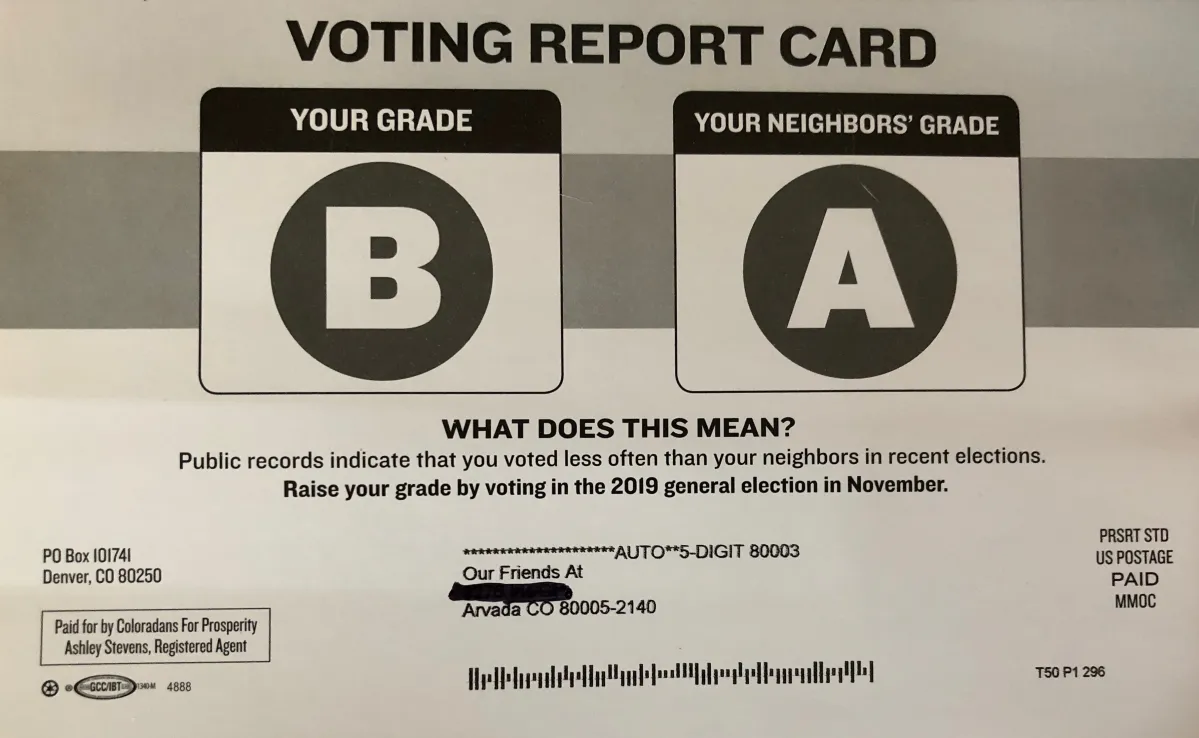
\includegraphics[width=0.5\textwidth,height=\textheight]{figs/socialpressure.png}

\pause

\begin{itemize}
\tightlist
\item
  \texttt{primary2004} whether the person voted in 2004, before the
  experiment. \pause
\item
  Do 2004 voters react differently to social pressure mailer than
  nonvoters? \pause
\item
  Two approaches: \pause

  \begin{itemize}
  \tightlist
  \item
    Subsets, subsets, subsets. \pause
  \item
    Interaction terms in regression.
  \end{itemize}
\end{itemize}
\end{frame}

\begin{frame}[fragile]{Subset approach}
\phantomsection\label{subset-approach}
\pause

\begin{itemize}
\tightlist
\item
  Easy way to estimate heterogeneous effects: our old friend,
  \texttt{filter()}, \texttt{group\_by()}, and \texttt{summarize()}.
  Woo! \pause

  \begin{itemize}
  \tightlist
  \item
    First, get the data
  \end{itemize}
\end{itemize}

\begin{Shaded}
\begin{Highlighting}[]
\FunctionTok{data}\NormalTok{(social, }\AttributeTok{package=}\StringTok{"qss"}\NormalTok{) }
\end{Highlighting}
\end{Shaded}
\end{frame}

\begin{frame}[fragile]{Subset approach}
\phantomsection\label{subset-approach-1}
\begin{itemize}
\tightlist
\item
  Now, estimate the ATE for the \textbf{voters}: \pause
\end{itemize}

\footnotesize

\begin{Shaded}
\begin{Highlighting}[]
\NormalTok{VotersATE }\OtherTok{\textless{}{-}}\NormalTok{ social }\SpecialCharTok{\%\textgreater{}\%}
  \FunctionTok{filter}\NormalTok{(primary2004 }\SpecialCharTok{==} \DecValTok{1}\NormalTok{,}
\NormalTok{         messages }\SpecialCharTok{\%in\%} \FunctionTok{c}\NormalTok{(}\StringTok{"Control"}\NormalTok{,}\StringTok{"Neighbors"}\NormalTok{)) }\SpecialCharTok{\%\textgreater{}\%}
  \FunctionTok{group\_by}\NormalTok{(messages) }\SpecialCharTok{\%\textgreater{}\%}
  \FunctionTok{summarize}\NormalTok{(}\AttributeTok{primary2006\_mean =} \FunctionTok{mean}\NormalTok{(primary2006)) }\SpecialCharTok{\%\textgreater{}\%}
  \FunctionTok{pivot\_wider}\NormalTok{(}\AttributeTok{names\_from =} \StringTok{"messages"}\NormalTok{,}
              \AttributeTok{values\_from =} \StringTok{"primary2006\_mean"}\NormalTok{) }\SpecialCharTok{\%\textgreater{}\%}
  \FunctionTok{mutate}\NormalTok{(}\AttributeTok{ate\_v =}\NormalTok{ Neighbors }\SpecialCharTok{{-}}\NormalTok{ Control) }\SpecialCharTok{\%\textgreater{}\%}
  \FunctionTok{select}\NormalTok{(ate\_v)}
\NormalTok{VotersATE}
\end{Highlighting}
\end{Shaded}

\begin{verbatim}
## # A tibble: 1 x 1
##    ate_v
##    <dbl>
## 1 0.0965
\end{verbatim}
\end{frame}

\begin{frame}[fragile]{Filter approach}
\phantomsection\label{filter-approach}
\begin{itemize}
\tightlist
\item
  Now, estimate the ATE for the \textbf{nonvoters}: \pause
\end{itemize}

\footnotesize

\begin{Shaded}
\begin{Highlighting}[]
\NormalTok{NonvotersATE }\OtherTok{\textless{}{-}}\NormalTok{ social }\SpecialCharTok{\%\textgreater{}\%}
  \FunctionTok{filter}\NormalTok{(primary2004 }\SpecialCharTok{==} \DecValTok{0}\NormalTok{,}
\NormalTok{         messages }\SpecialCharTok{\%in\%} \FunctionTok{c}\NormalTok{(}\StringTok{"Control"}\NormalTok{,}\StringTok{"Neighbors"}\NormalTok{)) }\SpecialCharTok{\%\textgreater{}\%}
  \FunctionTok{group\_by}\NormalTok{(messages) }\SpecialCharTok{\%\textgreater{}\%}
  \FunctionTok{summarize}\NormalTok{(}\AttributeTok{primary2006\_mean =} \FunctionTok{mean}\NormalTok{(primary2006)) }\SpecialCharTok{\%\textgreater{}\%}
  \FunctionTok{pivot\_wider}\NormalTok{(}\AttributeTok{names\_from =} \StringTok{"messages"}\NormalTok{,}
              \AttributeTok{values\_from =} \StringTok{"primary2006\_mean"}\NormalTok{) }\SpecialCharTok{\%\textgreater{}\%}
  \FunctionTok{mutate}\NormalTok{(}\AttributeTok{ate\_nv =}\NormalTok{ Neighbors }\SpecialCharTok{{-}}\NormalTok{ Control) }\SpecialCharTok{\%\textgreater{}\%}
  \FunctionTok{select}\NormalTok{(ate\_nv)}
\NormalTok{NonvotersATE}
\end{Highlighting}
\end{Shaded}

\begin{verbatim}
## # A tibble: 1 x 1
##   ate_nv
##    <dbl>
## 1 0.0693
\end{verbatim}
\end{frame}

\begin{frame}[fragile]{Difference in effects}
\phantomsection\label{difference-in-effects}
\begin{itemize}
\tightlist
\item
  How much does the estimated treatment effect differ between groups?
  \pause
\end{itemize}

\begin{Shaded}
\begin{Highlighting}[]
\NormalTok{VotersATE}\SpecialCharTok{$}\NormalTok{ate\_v }\SpecialCharTok{{-}}\NormalTok{ NonvotersATE}\SpecialCharTok{$}\NormalTok{ate\_nv}
\end{Highlighting}
\end{Shaded}

\begin{verbatim}
## [1] 0.02722908
\end{verbatim}

\pause

\begin{itemize}
\tightlist
\item
  Any easier way to allow for different effects of treatment by groups?
\end{itemize}
\end{frame}

\begin{frame}{Interaction terms}
\phantomsection\label{interaction-terms}
\pause

\begin{itemize}
\tightlist
\item
  Can allow for different effects of a variable with an interaction
  term: \pause
\end{itemize}

\[
\text{turnout}_i = \alpha + \beta_1\text{primary2004}_i + \beta_2\text{neighbors}_i + 
\] \[
\qquad \qquad \beta_3(\text{primary2004}_i \times \text{neighbors}_i) + \varepsilon_i
\]

\pause

\begin{itemize}
\tightlist
\item
  Primary 2004 variable multiplied by the neighbors variable.

  \begin{itemize}
  \tightlist
  \item
    Equal to 1 if voted in 2004 (primary2004 == 1) and received
    neighbors mailer (neighbors == 1) \pause
  \item
    Easiest to understand by investigating predicted values.
  \end{itemize}
\end{itemize}
\end{frame}

\begin{frame}{Predicted values from non-interacted model}
\phantomsection\label{predicted-values-from-non-interacted-model}
\pause

\begin{itemize}
\tightlist
\item
  Let \(X_i =\) primary2004\(_i\) and \(Z_i =\) neighbors\(_i\): \pause
\end{itemize}

\[
\hat{Y}_i = \hat{\alpha} + \hat{\beta}_1 X_i + \hat{\beta}_2 Z_i
\] \pause

\begin{center}
\begin{tabular}{ r | l  l }
 & Control ($Z_i = 0$) & Neighbors ($Z_i = 1$) \\
\hline
non-voter ($X_i = 0$)  & \only<3-10hu>{$\hat{\alpha}$} & \only<4-10>{$\hat{\alpha} + \hat{\beta}_2$} \\
voter ($X_i = 1$) & \only<5-10>{$\hat{\alpha} + \hat{\beta}_1$} & \only<6-10>{$\hat{\alpha} + \hat{\beta}_1 + \hat{\beta}_2$} \\
\end{tabular}
\end{center}

\begin{itemize}
\tightlist
\item
  \only<7-10>{Effect of Neighbors for non-voters:}
  \only<8-10>{$(\hat{\alpha} + \hat{\beta}_2) - (\hat{\alpha}) = \hat{\beta}_2$}
\item
  \only<9-10>{Effect of Neighbors for voters:}
  \only<10>{$(\hat{\alpha} + \hat{\beta}_1  + \hat{\beta}_2) - (\hat{\alpha} + \hat{\beta}_1) = \hat{\beta}_2$}
\end{itemize}
\end{frame}

\begin{frame}{Predicted from interacted model}
\phantomsection\label{predicted-from-interacted-model}
\begin{itemize}
\tightlist
\item
  Now for the interacted model:
\end{itemize}

\[
\hat{Y}_i = \hat{\alpha} + \hat{\beta}_1 X_i + \hat{\beta}_2 Z_i + \hat{\beta}_3 X_i Z_i
\]

\pause

\begin{center}
\begin{tabular}{ r | l  l }
 & Control ($Z_i = 0$) & Neighbors ($Z_i = 1$) \\
\hline
non-voter ($X_i = 0$)  & \only<2-5>{$\hat{\alpha}$} & \only<3-5>{$\hat{\alpha} + \hat{\beta}_2$} \\
voter ($X_i = 1$) & \only<4-5>{$\hat{\alpha} + \hat{\beta}_1$} & \only<5>{$\hat{\alpha} + \hat{\beta}_1 + \hat{\beta}_2 + \hat{\beta}_3$} \\
\end{tabular}
\end{center}
\end{frame}

\begin{frame}{Interpreting coefficients}
\phantomsection\label{interpreting-coefficients}
\[
\hat{Y}_i = \hat{\alpha} + \hat{\beta}_1\text{primary2004}_i + \hat{\beta}_2 \text{neighbors}_i 
\]

\[
\qquad \qquad \qquad \qquad + \hat{\beta}_3 (\text{primary2004}_i \times \text{neighbors}_i)
\] \pause 

\begin{center}
\begin{tabular}{ r | l  l }
 & Control Group & Neighbors Group \\
\hline
2004 primary non-voter  & $\hat{\alpha}$ & $\hat{\alpha} + \hat{\beta}_2  $ \\
2004 primary voter  & $\hat{\alpha} + \hat{\beta}_1$ & $\hat{\alpha} + \hat{\beta}_1 + \hat{\beta}_2 + \hat{\beta}_3$ \\
\end{tabular}
\end{center}
\pause

\begin{itemize}
\tightlist
\item
  \(\hat{\alpha}\): turnout rate for 2004 nonvoters in control group.
  \pause 
\item
  \(\hat{\beta}_1\): avg difference in turnout between 2004 voters and
  nonvoters. \pause 
\item
  \(\hat{\beta}_2\): effect of neighbors for 2004 nonvoters. \pause 
\item
  \(\hat{\beta}_3\): difference in the effect of neighbors mailer
  between 2004 voters and nonvoters.
\end{itemize}
\end{frame}

\begin{frame}[fragile]{Interactions in R}
\phantomsection\label{interactions-in-r}
\begin{itemize}
\tightlist
\item
  You can include an interaction with \texttt{var1}:\texttt{var2}:
\end{itemize}

\begin{Shaded}
\begin{Highlighting}[]
\NormalTok{social.neighbor }\OtherTok{\textless{}{-}}\NormalTok{ social }\SpecialCharTok{\%\textgreater{}\%}
  \FunctionTok{mutate}\NormalTok{(}\AttributeTok{neighbors =} \FunctionTok{ifelse}\NormalTok{(messages}\SpecialCharTok{==}\StringTok{"Neighbors"}\NormalTok{,}\DecValTok{1}\NormalTok{,}
                            \FunctionTok{ifelse}\NormalTok{(messages}\SpecialCharTok{==}\StringTok{"Control"}\NormalTok{,}\DecValTok{0}\NormalTok{,}\ConstantTok{NA}\NormalTok{))) }\SpecialCharTok{\%\textgreater{}\%}
  \FunctionTok{select}\NormalTok{(primary2006,primary2004,neighbors) }\SpecialCharTok{\%\textgreater{}\%}
  \FunctionTok{drop\_na}\NormalTok{()}
    
\NormalTok{fit }\OtherTok{\textless{}{-}} \FunctionTok{lm}\NormalTok{(primary2006 }\SpecialCharTok{\textasciitilde{}}\NormalTok{ primary2004 }\SpecialCharTok{+}\NormalTok{ neighbors }\SpecialCharTok{+}
\NormalTok{          primary2004}\SpecialCharTok{:}\NormalTok{neighbors, }\AttributeTok{data =}\NormalTok{ social.neighbor)}

\FunctionTok{coef}\NormalTok{(fit)}
\end{Highlighting}
\end{Shaded}

\begin{verbatim}
##           (Intercept)           primary2004 
##            0.23710990            0.14869507 
##             neighbors primary2004:neighbors 
##            0.06929617            0.02722908
\end{verbatim}
\end{frame}

\begin{frame}[fragile]{Interactions in R}
\phantomsection\label{interactions-in-r-1}
\begin{Shaded}
\begin{Highlighting}[]
\FunctionTok{coef}\NormalTok{(fit)}
\end{Highlighting}
\end{Shaded}

\begin{verbatim}
##           (Intercept)           primary2004 
##            0.23710990            0.14869507 
##             neighbors primary2004:neighbors 
##            0.06929617            0.02722908
\end{verbatim}

\pause

\begin{itemize}
\tightlist
\item
  Compare coefficients to earlier approach:
\end{itemize}

\begin{Shaded}
\begin{Highlighting}[]
\NormalTok{NonvotersATE}\SpecialCharTok{$}\NormalTok{ate\_nv}
\end{Highlighting}
\end{Shaded}

\begin{verbatim}
## [1] 0.06929617
\end{verbatim}

\pause

\begin{Shaded}
\begin{Highlighting}[]
\NormalTok{VotersATE}\SpecialCharTok{$}\NormalTok{ate\_v }\SpecialCharTok{{-}}\NormalTok{ NonvotersATE}\SpecialCharTok{$}\NormalTok{ate\_nv}
\end{Highlighting}
\end{Shaded}

\begin{verbatim}
## [1] 0.02722908
\end{verbatim}
\end{frame}

\end{document}
